\chapter{Metodología}\label{cap:metodo}

\section{Topología de referencia}
El laboratorio usa VirtualBox 7.2.22 sobre el equipo Windows del analista. Las cuatro VMs (1 vCPU y 1~GB de RAM cada una) y el anfitrión se conectan a una red solo-anfitrión. El adaptador NAT se usó únicamente para instalar paquetes y luego se deshabilitó (\cod{--nic1 none}); cada VM conserva solo \cod{enp0s8}, sin ruta por defecto. La Figura~\ref{fig:topologia} muestra la topología y la Tabla~\ref{tab:topologia}, el direccionamiento.

\begin{figure}[H]\centering
\begin{tikzpicture}[node distance=1.2cm,
  vm/.style={draw,rounded corners,fill=udazul!8,minimum width=2.8cm,minimum height=1.35cm,align=center,font=\small},
  host/.style={draw,rounded corners,fill=bgreal!10,minimum width=3.4cm,minimum height=1.35cm,align=center,font=\small}]
\node[vm] (gw) {\textbf{gateway} .1\\chrony (NTP) · nftables};
\node[vm,right=0.5cm of gw] (web) {\textbf{web} .20\\nginx :80};
\node[vm,right=0.5cm of web] (dns) {\textbf{dns} .53\\dnsmasq :53};
\node[vm,right=0.5cm of dns] (xmpp) {\textbf{xmpp} .30\\Prosody :5222/5269};
\coordinate (bus) at ($(gw.south)!0.5!(xmpp.south)+(0,-1.1)$);
\draw[very thick,black!60] ($(gw.south)+(-0.4,-1.1)$) -- ($(xmpp.south)+(0.4,-1.1)$) node[right,font=\scriptsize,align=left]{switch virtual\\solo-anfitrión};
\foreach \n in {gw,web,dns,xmpp}{\draw[thick] (\n.south) -- ++(0,-1.1);}
\node[host,below=1.9cm of $(web)!0.5!(dns)$] (an) {\textbf{analista} .10 (Windows)\\Wireshark 4.6.9 · Python 3.14.7};
\draw[thick] (an.north) -- (an.north |- bus);
\node[draw,dashed,rounded corners,inner sep=8pt,fit=(gw)(xmpp)(an),label={[font=\small\bfseries]above:Red aislada 192.168.50.0/24 — sin NAT ni ruta por defecto}] {};
\end{tikzpicture}
\caption{Topología del laboratorio. El gateway no reenvía tráfico (\texttt{ip\_forward = 0}): los peers de la subred se comunican directamente entre sí.}\label{fig:topologia}
\end{figure}

\begin{table}[H]\centering\small\caption{Direccionamiento y servicios por rol.}\label{tab:topologia}
\begin{tabularx}{\linewidth}{@{}lllX@{}}\toprule
\textbf{Rol} & \textbf{VM} & \textbf{IP} & \textbf{Servicios y configuración relevante}\\\midrule
gateway & lab-gateway & 192.168.50.1 & chrony servidor NTP (\cod{local stratum 10}); nftables con \cod{policy drop} en input y forward; \cod{ip\_forward = 0}\\
web & lab-web & 192.168.50.20 & nginx 1.24.0, HTTP :80 (\cod{HTTP/1.1 200 OK})\\
dns & lab-dns & 192.168.50.53 & dnsmasq 2.91, \cod{listen-address=192.168.50.53}, \cod{no-resolv}, \cod{web.lab.local → .20}\\
xmpp & lab-xmpp & 192.168.50.30 & Prosody 0.12.4, c2s :5222 y s2s :5269\\
analista & host Windows & 192.168.50.10 & Wireshark, Npcap, Python; DNS .53; regla de firewall para ICMP desde la subred\\
\bottomrule\end{tabularx}\end{table}

El firewall del gateway (Figura~\ref{fig:gwfw}) descarta por defecto y solo acepta loopback, tráfico establecido y gestión ICMP, NTP y SSH desde la red del laboratorio:

\begin{lstlisting}
table inet filter {
  chain input {
    type filter hook input priority 0; policy drop;
    iif lo accept
    ct state established,related accept
    ip saddr 192.168.50.0/24 icmp type echo-request accept
    ip saddr 192.168.50.0/24 udp dport 123 accept
    ip saddr 192.168.50.0/24 tcp dport 22 accept
  }
  chain forward { type filter hook forward priority 0; policy drop; }
}
\end{lstlisting}

\section{Herramientas}
\begin{table}[H]\centering\small\caption{Herramientas y versiones utilizadas.}\label{tab:herramientas}
\begin{tabularx}{\linewidth}{@{}lp{3.1cm}X@{}}\toprule
\textbf{Herramienta} & \textbf{Versión} & \textbf{Uso}\\\midrule
VirtualBox & 7.2.22 (r175245) & Hipervisor, snapshots \cod{lab-base-aislado-v2}\\
Ubuntu Server & 24.04.5 LTS, kernel 6.8.0-149 & Sistema de las cuatro VMs\\
chrony & 4.5-1ubuntu4.2 & Servidor y clientes NTP\\
nftables & 1.0.9 & Firewall del gateway y validación de reglas propuestas (\cod{nft -c})\\
nginx · dnsmasq · Prosody & 1.24.0 · 2.91 · 0.12.4 & Servicios web, DNS y XMPP\\
Wireshark · Npcap & 4.6.9 · 1.90 & Captura y visualización en el analista\\
tshark & 4.6.9 (analista); 4.2.2 (re-ejecución) & Extracción de campos desde los scripts\\
Python & 3.14.7 (analista); 3.13 (re-ejecución) & Generadores, analizadores, pipeline y Parte II\\
scikit-learn · pandas · matplotlib & 1.9.1 · 3.1.1 · 3.11.2 & Caso 4 y gráficas\\
OpenSSL & 3.5.7 (cliente) · 3.0.13 (servidor) & Pruebas STARTTLS del Caso 10\\
FastAPI · SQLAlchemy · Leaflet & 0.165 · 2.1.9 · 1.9.4 & Parte II\\
Google Chrome + Playwright & — & Prueba de extremo a extremo y capturas de la Parte II\\
\bottomrule\end{tabularx}\end{table}

No se instalaron Suricata, Zeek ni Wazuh: la guía los presenta como opcionales y las VMs no tienen salida a Internet. Las reglas de detección se expresan como reglas nftables y como lógica en Python, y la correlación del Caso~9 usa un pipeline propio equivalente en sus etapas a un SIEM (sección~\ref{sec:caso9}).

\section{Sincronización de relojes}
La correlación entre fuentes exige relojes coherentes. El gateway sirve hora con chrony a la subred; web, dns y xmpp lo usan como única fuente (\cod{chronyc sources} muestra \cod{\^{}* 192.168.50.1}) y el analista Windows lo consulta con w32time (\cod{Origen: 192.168.50.1}, capa 4). Todas las VMs reportan \cod{System clock synchronized: yes} y zona \cod{America/Bogota}.

\section{Verificación del laboratorio}
Se ejecutó \cod{verificar\_laboratorio.sh <rol>} en cada VM, antes y después de retirar el NAT, y \cod{verificar\_laboratorio.ps1 -Rol analista} en el anfitrión: 11 comprobaciones correctas, ninguna faltante y una advertencia (Wireshark instalado pero fuera del PATH, luego corregida en el script). Estas comprobaciones verifican conectividad y servicios; no son una auditoría integral de seguridad. El ping sin respuesta a 192.0.2.1 (TEST-NET) es un indicio auxiliar de aislamiento, no una prueba por sí solo; la prueba es la ausencia del adaptador NAT y de ruta por defecto.

\fig[0.62]{gateway-aislado-crop.png}{Gateway tras el retiro del NAT: solo \texttt{lo} y \texttt{enp0s8}, una única ruta a 192.168.50.0/24 y el ruleset nftables cargado.}
\begin{figure}[H]\centering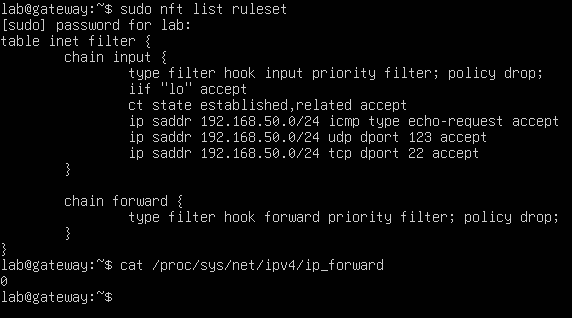
\includegraphics[width=0.58\linewidth]{fig/gateway-firewall-crop.png}\caption{Ruleset del gateway con \texttt{policy drop} e \texttt{ip\_forward = 0}.}\label{fig:gwfw}\end{figure}
\fig[0.95]{web-nginx-crop.png}{Servidor web: nginx activo y respuesta \texttt{HTTP/1.1 200 OK} (captura tomada durante el montaje, todavía con el adaptador NAT \texttt{enp0s3}).}
\fig[0.95]{dns-resolucion-crop.png}{DNS: \texttt{web.lab.local} resuelve a 192.168.50.20 en dnsmasq (captura del montaje, con NAT aún presente).}
\fig[0.95]{xmpp-prosody-crop.png}{XMPP: Prosody activo y escuchando en 5222 (IPv4 e IPv6).}
\fig[0.62]{web-ntp-crop.png}{Cliente NTP: la VM web sincroniza contra el gateway (\texttt{\^{}* 192.168.50.1}, \texttt{Reference ID C0A83201}).}
\begin{figure}[H]\centering
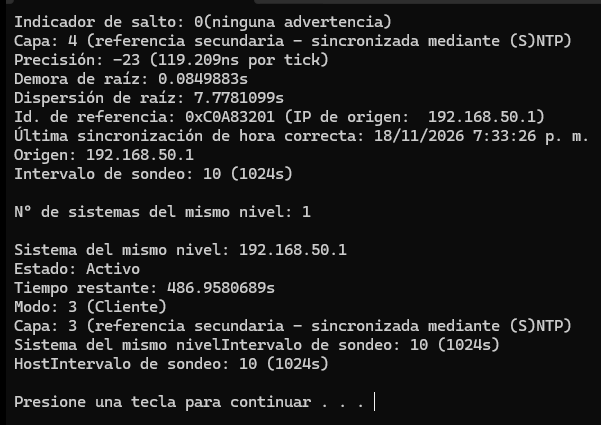
\includegraphics[width=0.48\linewidth]{fig/host-w32tm-crop.png}\hfill
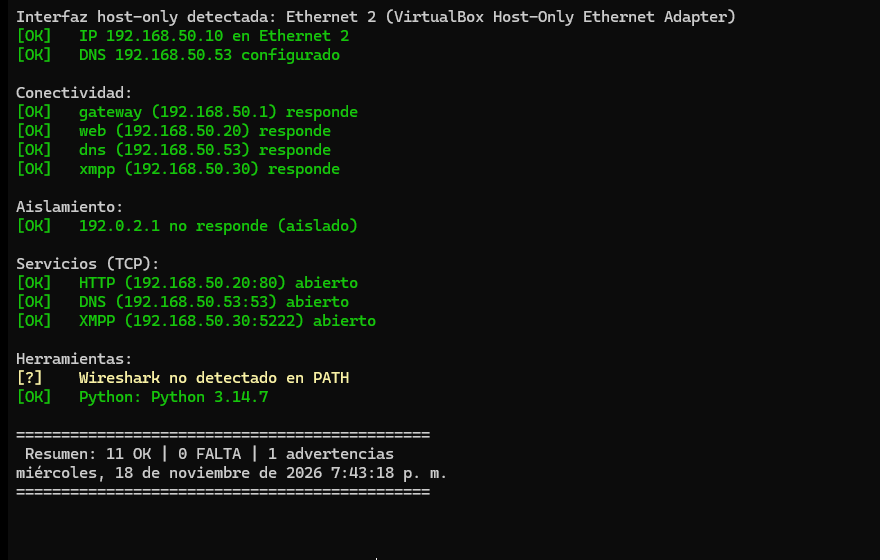
\includegraphics[width=0.48\linewidth]{fig/host-verificacion-analista-crop.png}
\caption{Analista Windows: w32time con origen 192.168.50.1 (izquierda) y verificación del rol analista con 11 OK, 0 FALTA y 1 advertencia (derecha).}\end{figure}
\fig{host-wireshark.png}{Captura en vivo en Wireshark sobre el adaptador \emph{Ethernet 2}: tráfico ICMP, TCP/HTTP, DNS y ARP del propio laboratorio.}

\section{Método de evidencia y reproducibilidad}\label{sec:metodo-evidencia}
\paragraph{Integridad.} Cada archivo se registra con SHA-256 (además de SHA-1 y MD5 por compatibilidad) en \cod{evidencia.log} con \cod{hash\_evidencia.py}. Al cerrar la Parte~I, \cod{scripts/cerrar\_parte\_i.py} copió 242 archivos a dos copias, \cod{original} y \cod{trabajo}, y generó un manifiesto JSON con ruta, tamaño y SHA-256 de cada uno, más la huella del propio manifiesto. La verificación recalcula todo y falla si un solo byte cambia.

\paragraph{Saltos de línea.} Git convirtió CRLF a LF los archivos de texto confirmados desde Windows, de modo que el manifiesto no verificaba en un clon. Se añadió \cod{.gitattributes} para guardar la evidencia byte a byte y \cod{scripts/reparar\_evidencia.py} restauró los CRLF originales. Cuatro archivos con saltos mixtos (\cod{caso03-auth-events}, \cod{caso03-ss-tulpn}, \cod{caso05-logs-correlacion} y \cod{caso06-openresolver}) no se podían reproducir; el manifiesto los registra en una lista de \emph{enmiendas} con su huella original, la actual y el motivo. Desde el commit \cod{02257d9} la verificación pasa en un clon limpio (Figura~\ref{fig:integridad}).

\paragraph{Reproducción.} Para este informe se clonó \cod{main} y se re-ejecutaron los analizadores sobre las mismas PCAP: las salidas de los casos 1, 2, 5, 6, 7 y 8 son idénticas byte a byte a las conservadas y las métricas del Caso~4 coinciden. Las capturas de terminal del capítulo~\ref{cap:parte1} provienen de esa re-ejecución.

\begin{figure}[H]\centering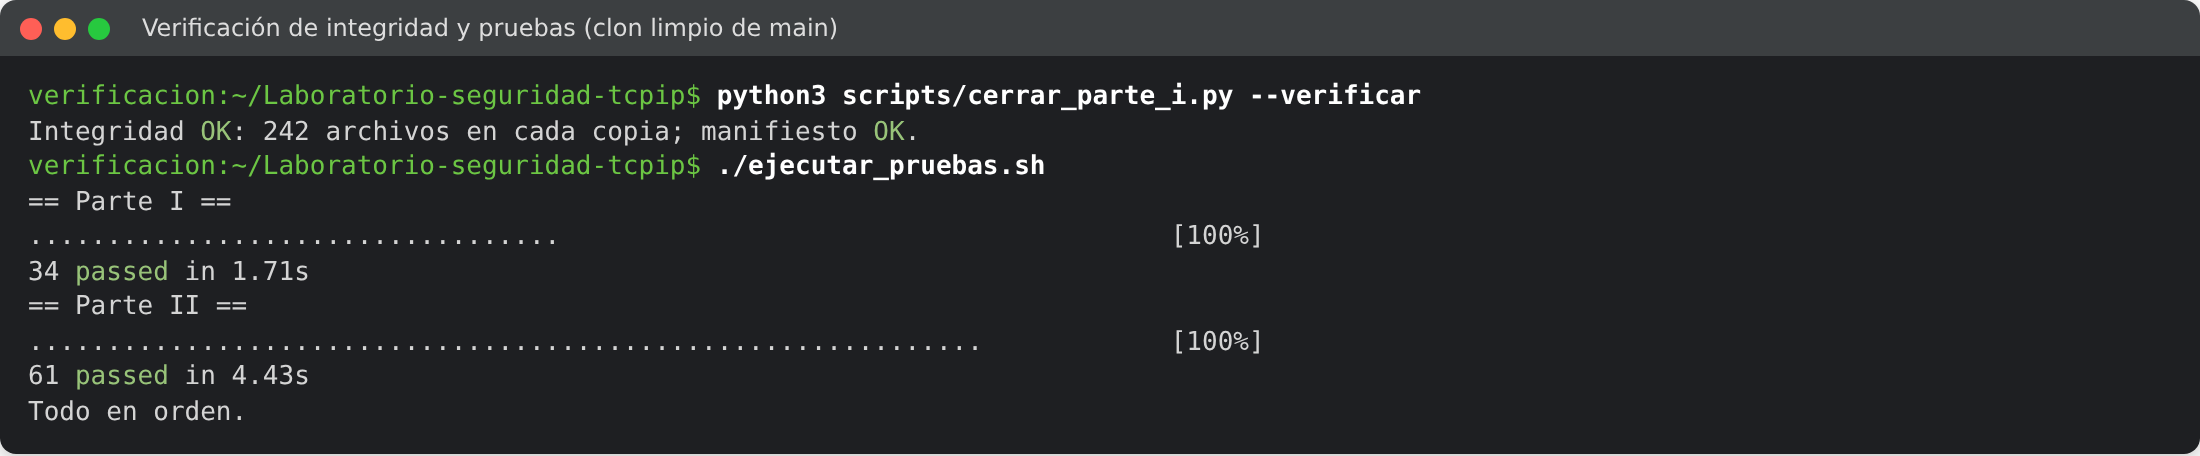
\includegraphics[width=\linewidth]{fig/term-integridad.png}
\caption{Verificación del manifiesto (242 archivos por copia) y ejecución de las pruebas de la Parte I (34) y la Parte II (61) en un clon limpio.}\label{fig:integridad}\end{figure}

\paragraph{Línea base.} \cod{baseline-normal.pcapng} (1.639 paquetes, 296,67~s) es tráfico real capturado en el analista, pero incluye ruido del propio Windows: consultas DNS a dominios externos, mDNS, LLMNR y NBNS. Se generó \cod{baseline-normal-limpia.pcapng} (720 paquetes, 293,26~s) conservando solo IPv4 dentro de 192.168.50.0/24 sin esos protocolos. La original se mantiene porque los casos cerrados verifican su huella; los casos 1, 4 y 7 se repitieron sobre la limpia (capítulo~\ref{cap:discusion}).

\fig{term-baseline.png}{Líneas base original y limpia: número de paquetes, duración y SHA-256.}

\section{Formato mínimo de registro por hallazgo}
Cada caso se documenta con una ficha de nueve campos. Como no se dispuso del apartado literal de la plantilla de la guía, se adoptó la estructura de la Tabla~\ref{tab:formato} y se declara como propuesta.

\begin{table}[H]\centering\small\caption{Campos de la ficha de registro por hallazgo.}\label{tab:formato}
\begin{tabularx}{\linewidth}{@{}p{3.2cm}X@{}}\toprule
\textbf{Campo} & \textbf{Contenido}\\\midrule
Identificador & Código del caso (CASO-01 a CASO-10)\\
Título & Hallazgo en una frase, sin afirmar más de lo demostrado\\
Fecha y analista & Fecha de ejecución y zona horaria; las marcas UTC se convierten a UTC$-$05:00\\
Categoría & Tipo de amenaza o técnica y si es estudio, simulación o incidente\\
Descripción & Qué se observó, con origen, destino y volúmenes\\
Severidad & Potencial y efectiva, separadas; criterio de impacto\\
Evidencias & Archivos con su huella en el manifiesto\\
Observables & Valores medidos que sostienen el hallazgo y el filtro usado\\
Estado & Qué queda confirmado y qué no; acciones pendientes\\
\bottomrule\end{tabularx}\end{table}

Además, cada caso incluye el procedimiento reproducible, la regla de detección o mitigación propuesta con su ubicación correcta en la red y preguntas de análisis.
